\section{Modèle}

\subsection{Diagramme de classes}

\paragraph{}
La figure \ref{fig:class} présente le diagramme de classe général élaboré pour le projet.
Nous avons fait nos choix de modélisation de façon à avoir le moins de classes possibles, tout en restant dans la simplicité.
Certains choix ont été effectués de façon à introduire les patrons de conception requis pour le projet. Ces choix seront présentés dans la partie suivante.

\paragraph{}
Le diagramme présenté va subir inévitablement des changements lors du développement du projet. Cependant, la structure générale ne devrait pas être amenée à changer. Des diagrammes de séquence seront présentés en partie \ref{diagSequence} afin de conforter nos choix de modélisations.

\begin{figure}[h]
  \centering
  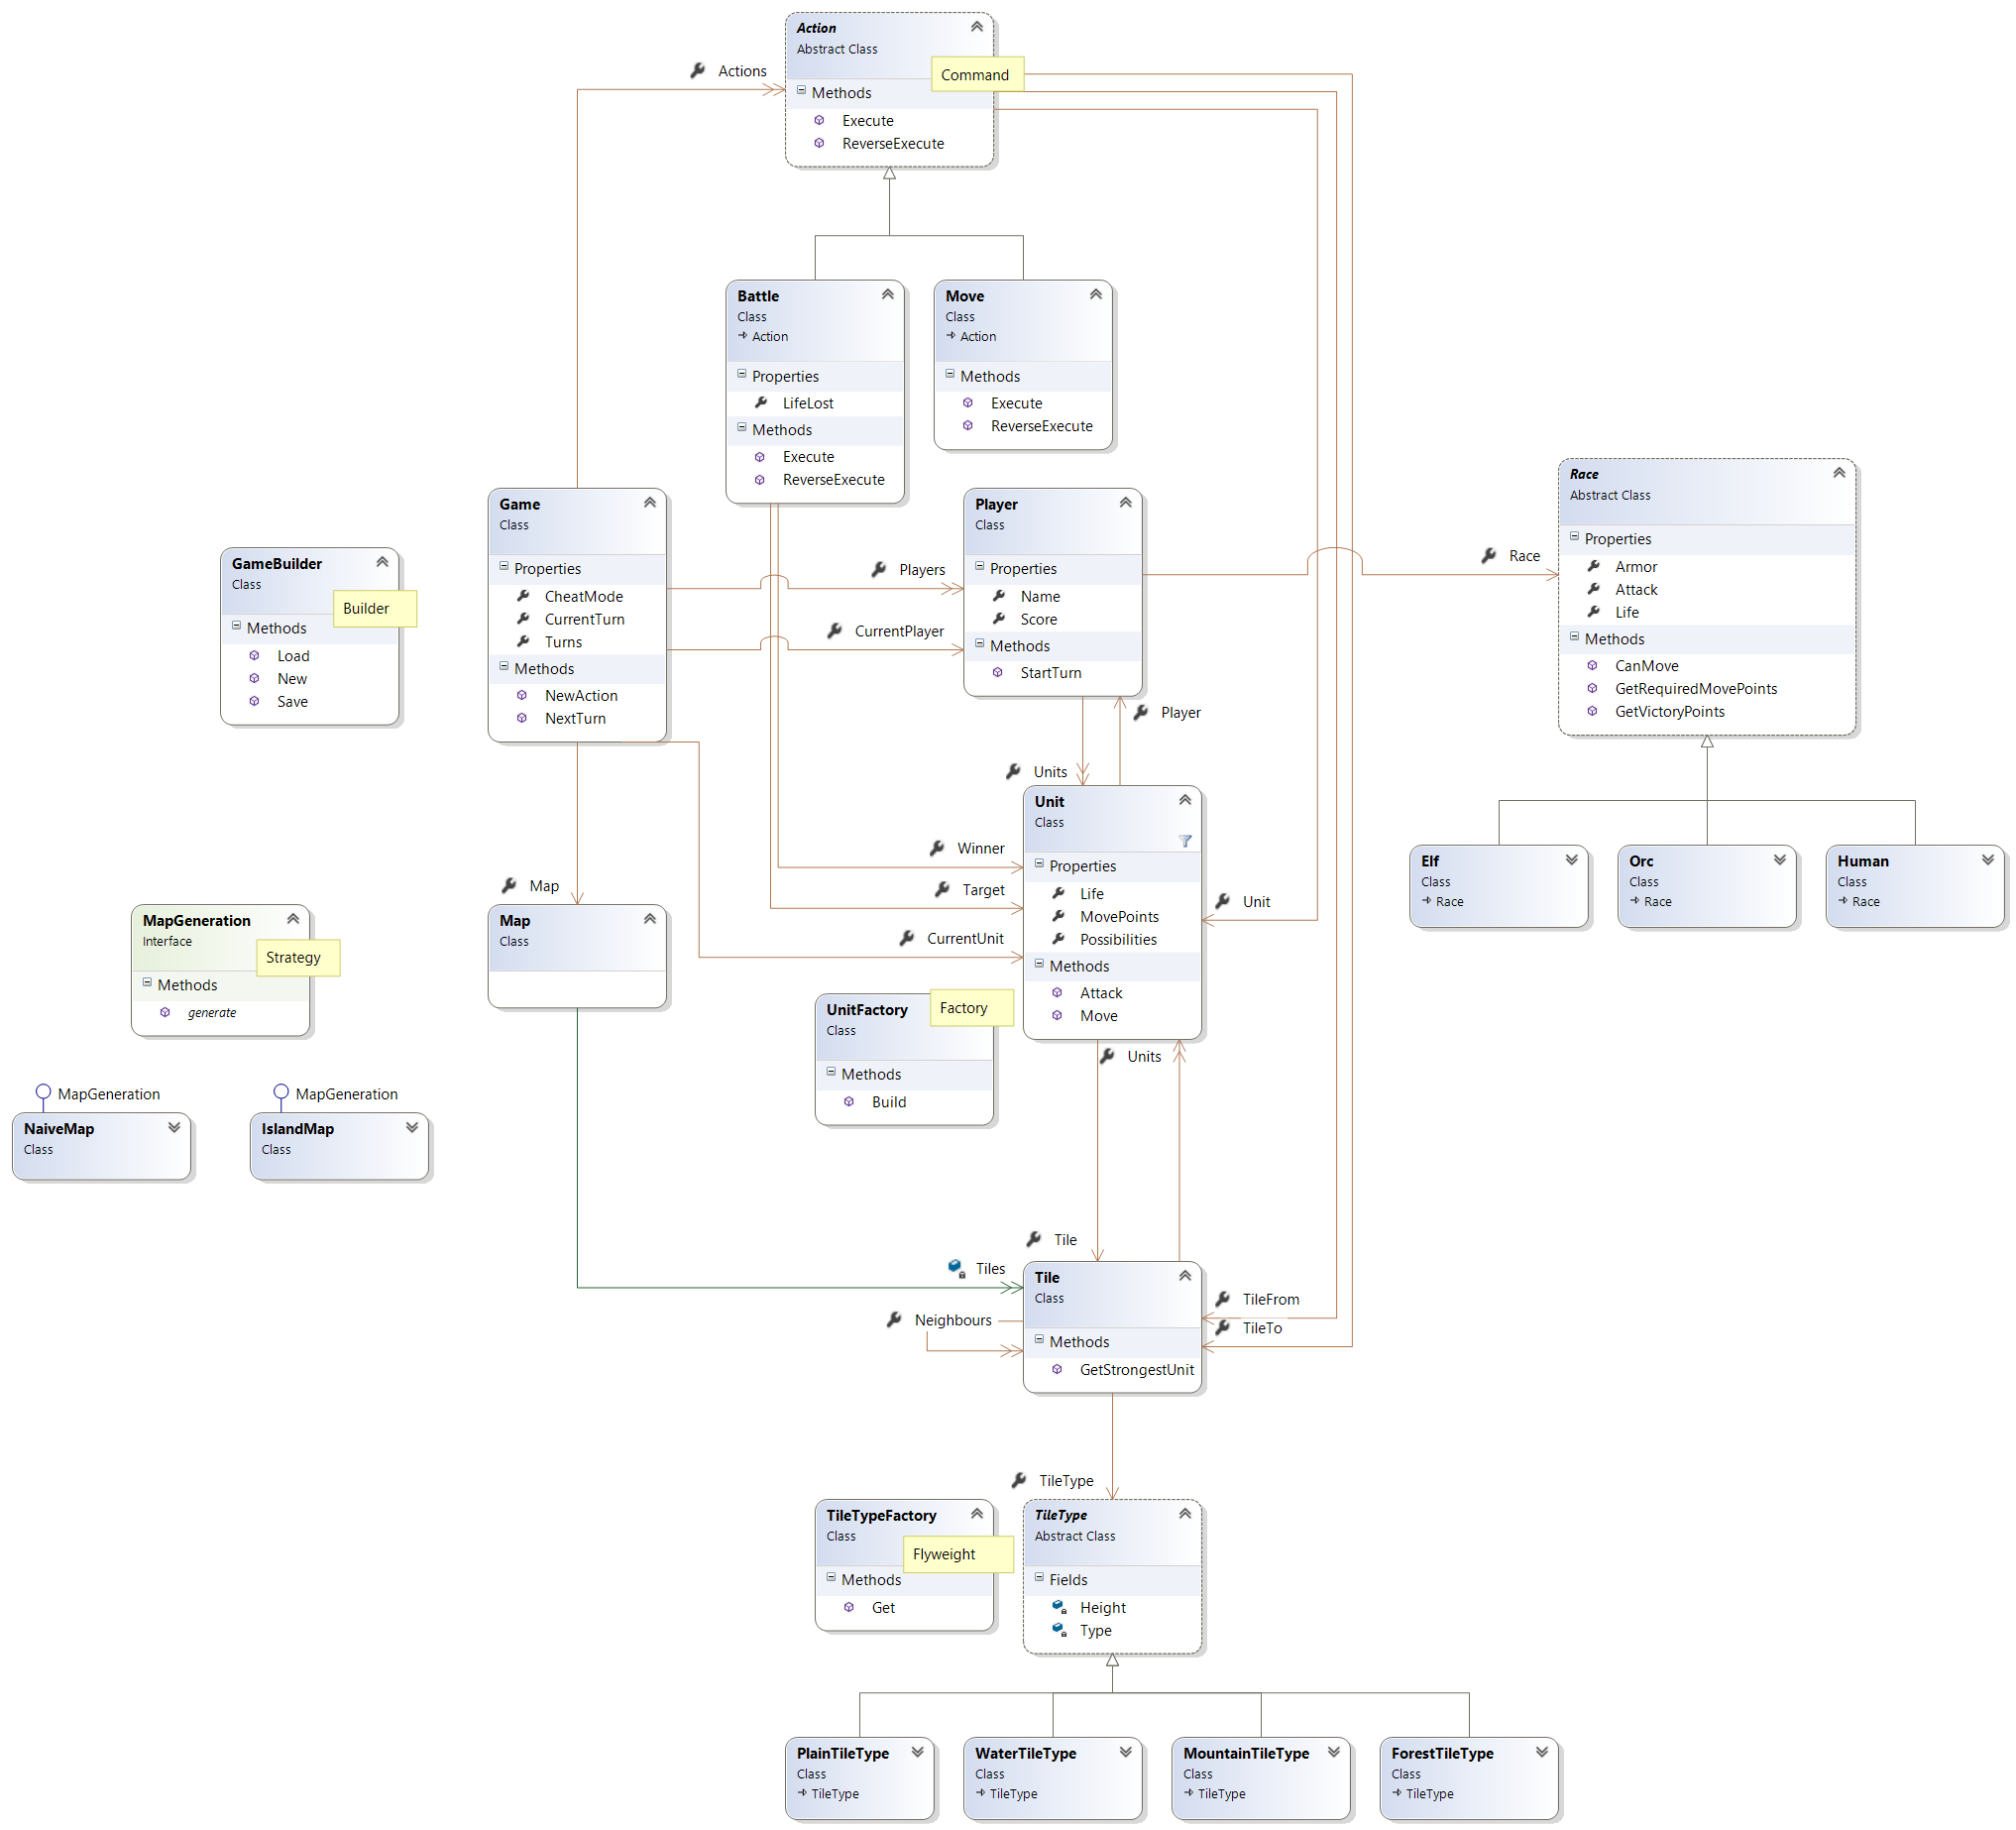
\includegraphics[width=13cm]{schemas/ClassDiagram.png}
  \caption{Diagramme de classes général}
  \label{fig:class}
\end{figure}

\subsection{Patrons de conception}

\paragraph{}
Les différents patrons de conception utilisés dans le projet vont être présentés dans cette partie.

\subsubsection{Génération de carte : Stratégie}

\paragraph{}
Nous avons choisi d'implémenter une Stratégie pour la \textbf{génération de la carte}.
En effet, nous prévoyons d'implémenter plusieurs algorithmes de génération, choisis aléatoirement ou par choix utilisateur parmi la liste non exhaustive suivante :

\begin{itemize}
  \item Génération naïve : il s'agit d'une génération parfaitement aléatoire
  \item Génération d'une île
  \item Génération d'un cratère de volcan
\end{itemize}

Ces algorithmes seront probablement développés en C++ pour acroître la rapidité de leur exécution.
Leur nombre sera défini par le temps restant pour les développer.

\paragraph{}
Le patron Stratégie, présenté dans la figure \ref{fig:strategy}, a été choisi pour sa capacité à exécuter une action de plusieurs façon différentes.

\begin{figure}[h]
  \centering
  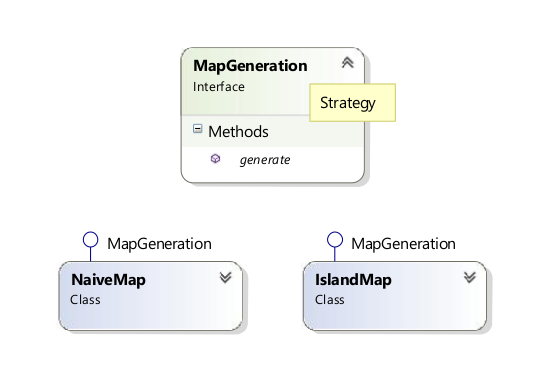
\includegraphics[width=13cm]{schemas/dp_strategy.png}
  \caption{Patron de conception Stratégie}
  \label{fig:strategy}
\end{figure}

\subsubsection{Gestion des types de case : Poids-Mouche}

\paragraph{}
Chaque case de la carte étant d'un type parmi 4, nous avons choisi de modéliser les classes représentant les types de cases via un Poids-Mouche.
En effet, beaucoup de cases feront référence au même type, il n'est donc pas nécessaire d'instancier plusieurs fois le même type, ayant à chaque fois les mêmes caractéristiques.
Ce cas de figure correspond parfaitement au Poids-Mouche, bien que le nombre de cases à gérer soit relativement faible. Il est présenté dans la figure \ref{fig:flyweight}.
L'obtention d'un type de case se fait via la classe \emph{TileTypeFactory} (méthode \emph{Get(String type)}). Si une instance du type demandé existe, elle est retournée directement.
Sinon, elle est créée puis retournée.

\paragraph{}
Nous aurions pu également utiliser des classes comportant des informations statiques, ou bien des énumérations pour gagner en simplicité et rapidité.
L'utilisation d'un Poids-Mouche est donc principalement choisie dans un objectif pédagogique.

\begin{figure}[h]
  \centering
  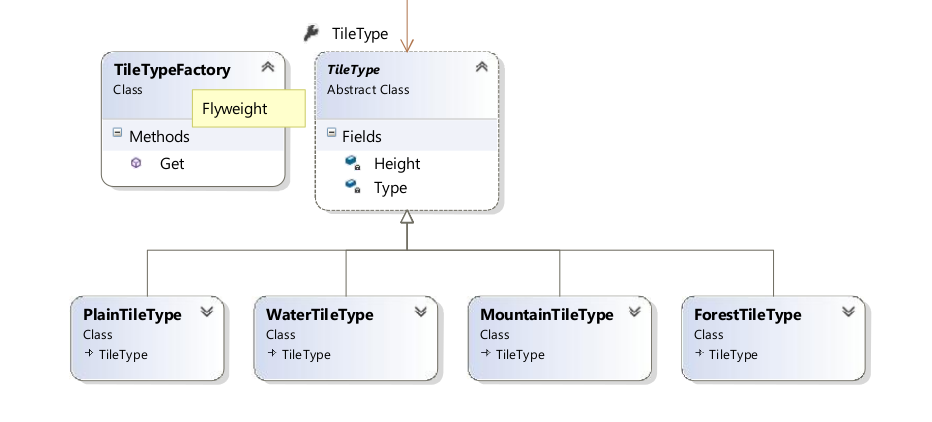
\includegraphics[width=13cm]{schemas/dp_flyweight.png}
  \caption{Patron de conception Poids-Mouche}
  \label{fig:flyweight}
\end{figure}

\subsubsection{Création d'une unité : Fabrique}

\paragraph{}
La création d'une unité pouvant se révéler fastidieuse, nous avons décidé de réaliser une Fabrique d'unités, nommée \emph{Unit Factory}.
Dans la pratique, cette fabrique sera chargée d'initialiser correctement les points de vie d'une unité en fonction de sa race et de mettre à jour sa position sur la carte.
La figure \ref{fig:factory} présente cette fabrique simple.

\begin{figure}[h]
  \centering
  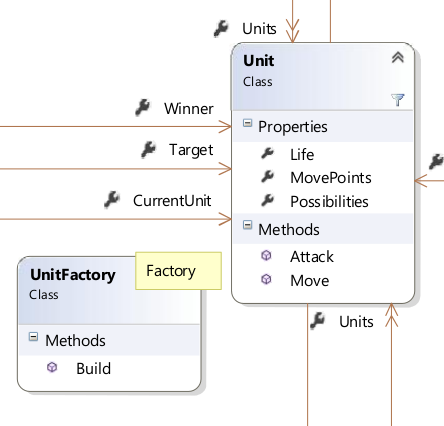
\includegraphics[width=8cm]{schemas/dp_factory.png}
  \caption{Patron de conception Fabrique}
  \label{fig:factory}
\end{figure}

\subsubsection{Initialisation d'une partie : Constructeur}

\paragraph{}
De manière similaire à la fabrique présentée, il est complexe d'initialiser une partie.
Nous avons donc mis en place le patron Constructeur pour gérer cette initialisation, en plusieurs étapes.
Ce constructeur est chargé d'initialiser la carte, de créer les unités et de préparer le démarrage du jeu.

\paragraph{}
Il sera possible de créer une nouvelle partie, ou d'utiliser un fichier de sauvegarde pour relancer une partie interrompue, et ce via les méthodes \emph{New} et \emph{Load} du Constructeur \emph{GameBuilder}.
Le fonctionnement détaillé de l'initialisation d'une partie est détaillé dans la figure \ref{fig:sd_init}, et le schéma du Constructeur est disponible en tant que figure \ref{fig:builder}.

\begin{figure}[h]
  \centering
  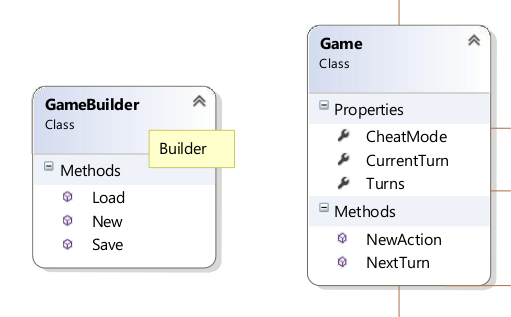
\includegraphics[width=8cm]{schemas/dp_builder.png}
  \caption{Patron de conception : Constructeur}
  \label{fig:builder}
\end{figure}

\subsubsection{Annulation d'une action : Commande / Memento}

\paragraph{}
Enfin, nous avons utilisé le patron Commande, associé au patron Memento et présenté dans la figure \ref{fig:command}.
L'objectif de cette structure est la \textbf{conservation des actions effectuées} par les joueurs au cours de la partie, afin d'être capable d'inverser ces actions (quand un mode triche est activé).
Les deux actions possibles (attaque et mouvement) contiennent les informations nécessaires à leur inversion, et la liste des actions effectuées sera stockée dans la classe \emph{Game}.

\paragraph{}
Le fonctionnement de ce patron étant assez subtil, un diagramme de séquence est disponible dans le cas d'une bataille en figure \ref{fig:sd_battle}.

\begin{figure}[h]
  \centering
  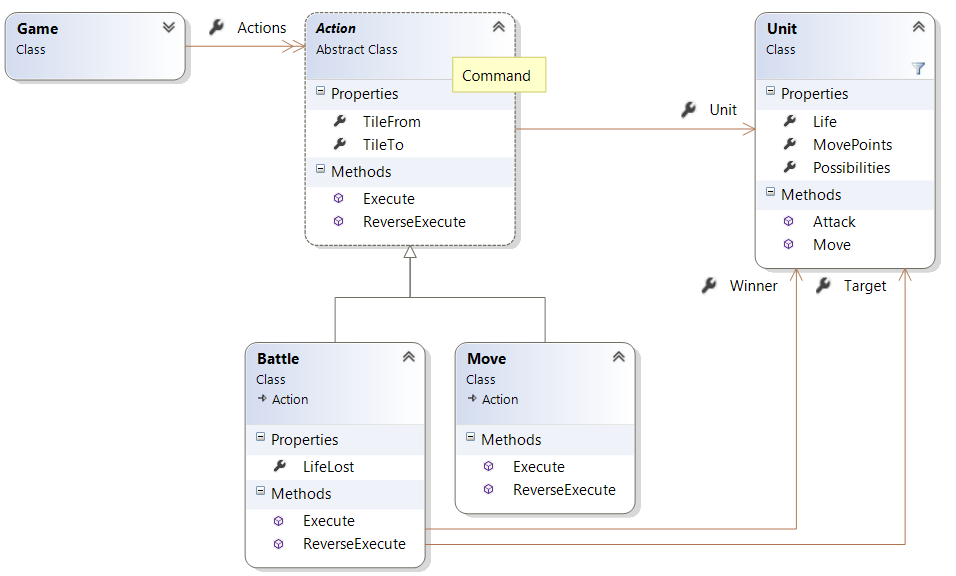
\includegraphics[width=13cm]{schemas/dp_command.png}
  \caption{Patron de conception : Commande / Memento}
  \label{fig:command}
\end{figure}

\subsection{Diagrammes de séquence}
\label{diagSequence}
\subsubsection{Initialisation d'une nouvelle partie}

\begin{figure}[h]
  \centering
  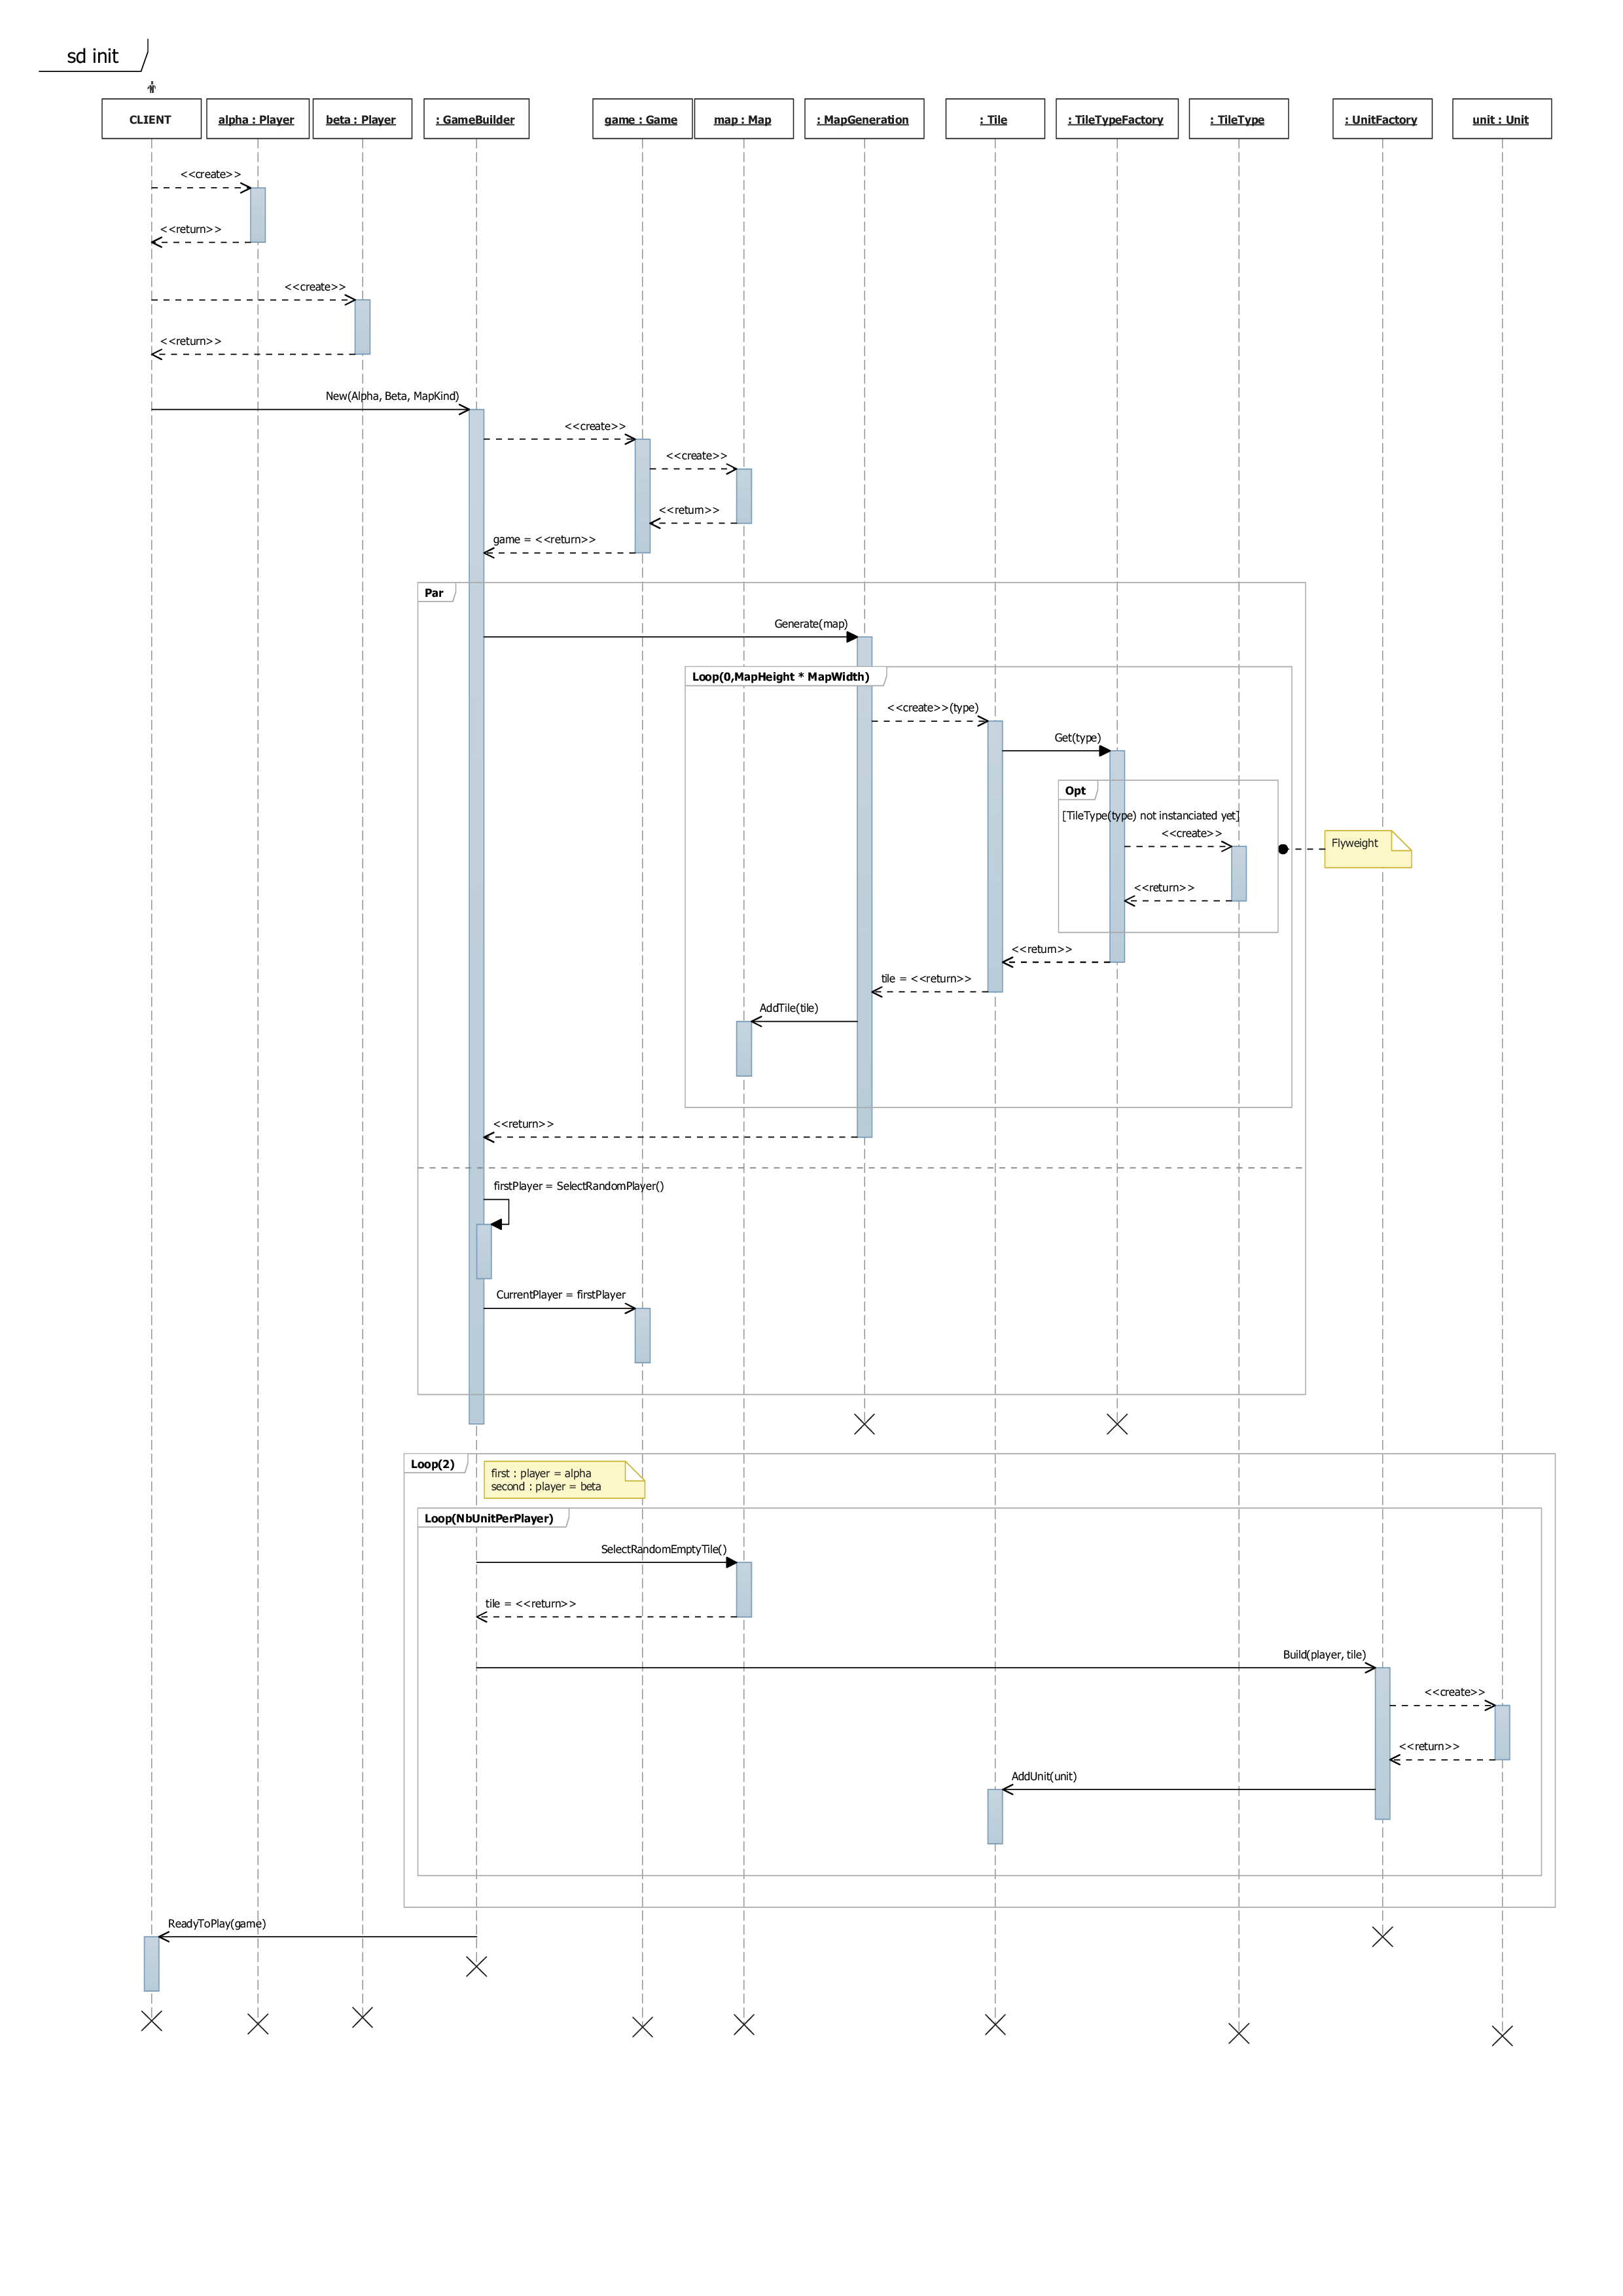
\includegraphics[width=13cm]{schemas/sd_init.png}
  \caption{Diagramme de séquence de l'initialisation du jeu}
  \label{fig:sd_init}
\end{figure}

\subsubsection{Bataille}

\begin{figure}[h]
  \centering
  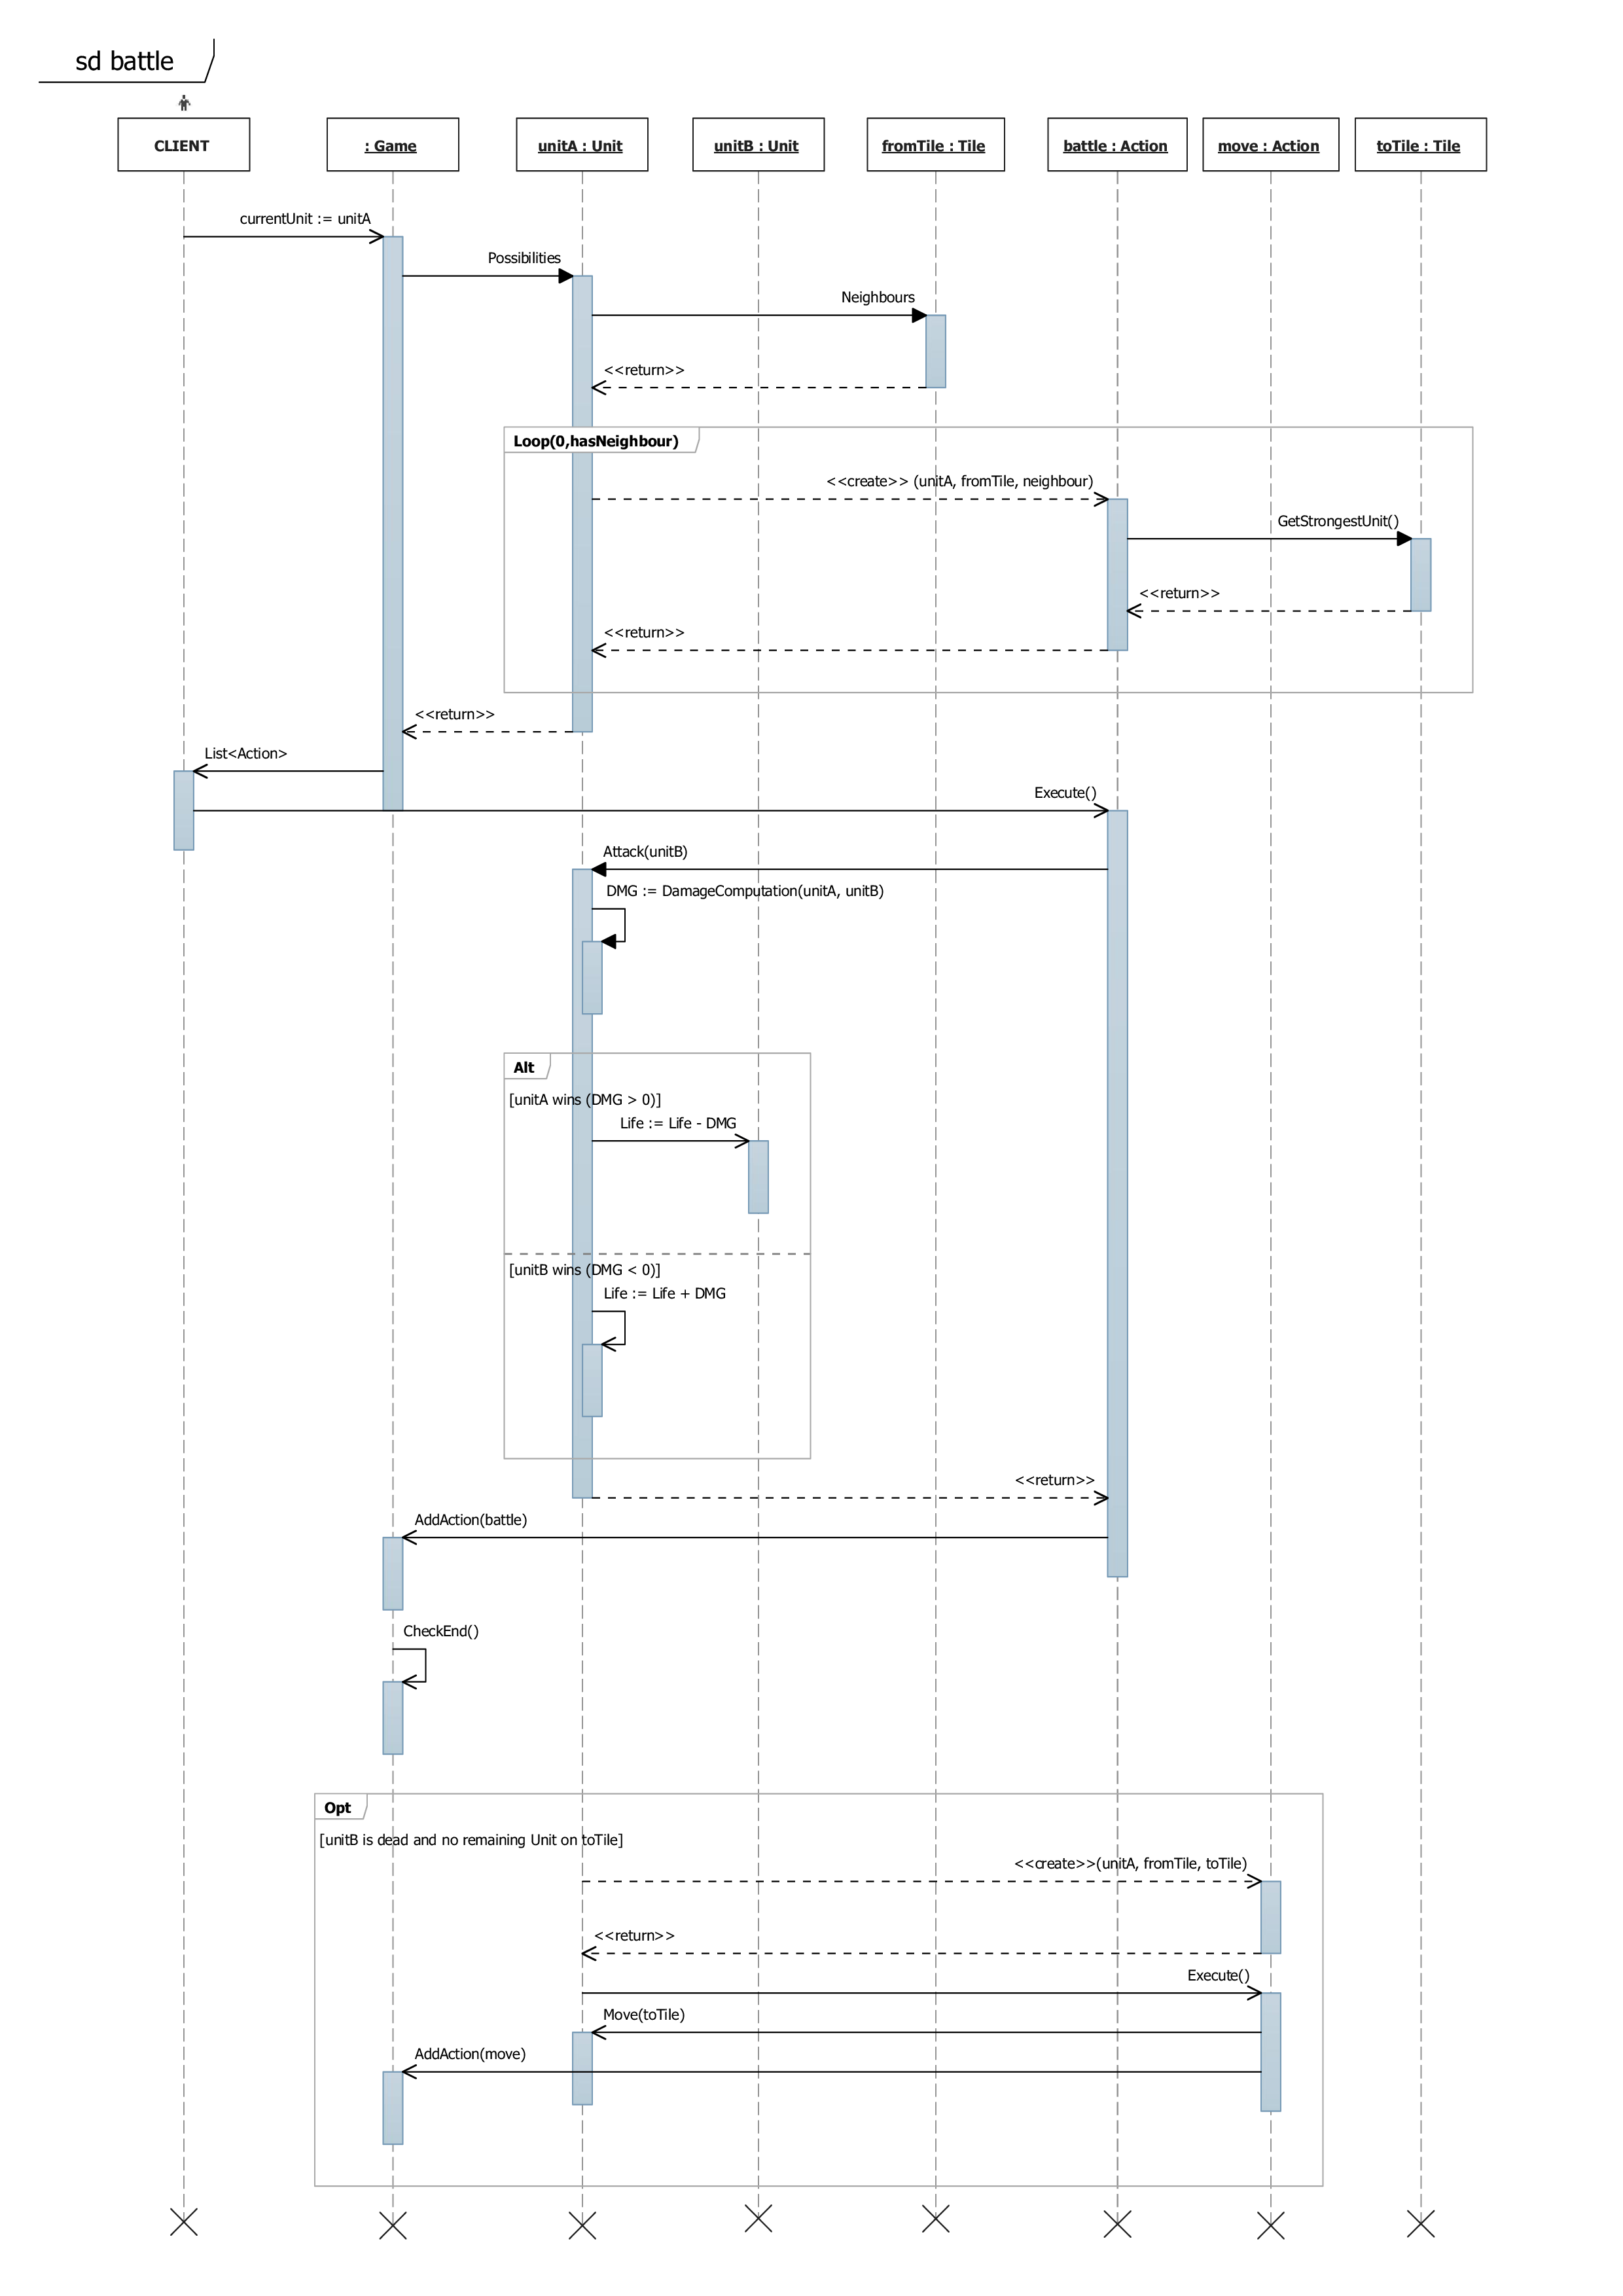
\includegraphics[width=13cm]{schemas/sd_battle.png}
  \caption{Diagramme de séquence d'une bataille}
  \label{fig:sd_battle}
\end{figure}
